\documentclass[12pt,fleqn]{article}\usepackage{../common}
\begin{document}

\begin{minted}[fontsize=\footnotesize]{python}
import pandas as pd
df = pd.read_csv('oilprice.csv',header=None,index_col=0)
pd.rolling_mean(df[1],40).plot()
plt.savefig('corr_01.png')
\end{minted}

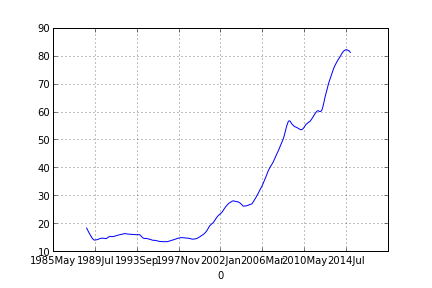
\includegraphics[height=6cm]{corr_01.png}

\begin{minted}[fontsize=\footnotesize]{python}
print len(list(pd.rolling_mean(df[1],80).dropna()))
\end{minted}

\begin{verbatim}
276
\end{verbatim}

\begin{minted}[fontsize=\footnotesize]{python}
import pandas as pd
import datetime
from dateutil.parser import parse
price = pd.read_csv('oilprice.csv',header=None,index_col=0)
prod = pd.read_csv('world.csv',parse_dates=True,index_col=0,sep=' ')
price.index = map(lambda x: datetime.datetime.strptime(x,'%Y%b'), price.index)
prod['price'] = price
print prod.price.corr(prod.oil)
\end{minted}

\begin{verbatim}
0.812066270665
\end{verbatim}

\begin{minted}[fontsize=\footnotesize]{python}
prod.plot()
plt.savefig('corr_02.png')
\end{minted}

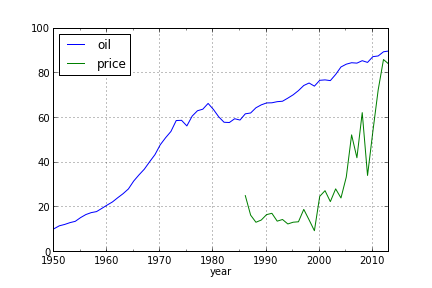
\includegraphics[height=6cm]{corr_02.png}

\begin{minted}[fontsize=\footnotesize]{python}
import pandas as pd
df = pd.read_csv('burgersold.csv',sep=' ',header=None,index_col=0,names=['sold'])
df['price'] = pd.read_csv('burgerprice.csv',sep=' ',header=None,index_col=0)
df['price'] = df['price'].interpolate()
df['inflation'] = pd.read_csv('usinf.csv',index_col=0,sep='\s*')
df['adjprice'] = df['price'] / (1 + (df['inflation'] / 100.)).cumprod()
print df.sold.corr(df.adjprice)
\end{minted}

\begin{verbatim}
0.445384371682
\end{verbatim}

http://the-american-catholic.com/2014/11/21/wages-and-hamburgers-a-pricing-history/

\begin{minted}[fontsize=\footnotesize]{python}
df['price'].plot()
plt.savefig('corr_03.png')
\end{minted}

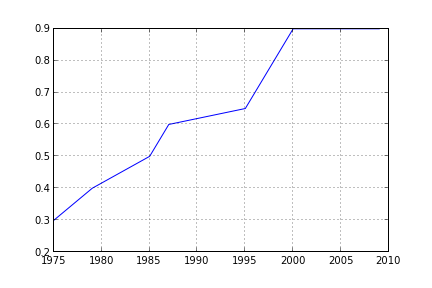
\includegraphics[height=6cm]{corr_03.png}


\begin{minted}[fontsize=\footnotesize]{python}
df['sold'].plot()
plt.savefig('corr_04.png')
\end{minted}

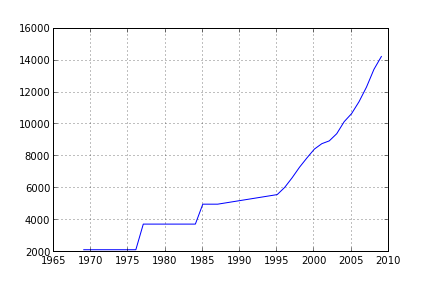
\includegraphics[height=6cm]{corr_04.png}


\begin{minted}[fontsize=\footnotesize]{python}
import pandas as pd, re
df = pd.read_csv('oilprice.csv')
df['year'] = df['date'].map(lambda x: int(re.search(r'(\d+)',x).groups(1)[0]))
df = df.drop('date',axis=1).groupby('year').mean()
df['inflation'] = pd.read_csv('usinf.csv',index_col=0,sep='\s*')
df['inflation adjusted oil price'] = df['price'] / (1 + (df['inflation'] / 100.)).cumprod()
df[['price','inflation adjusted oil price']].plot()
plt.savefig('corr_05.png')
\end{minted}

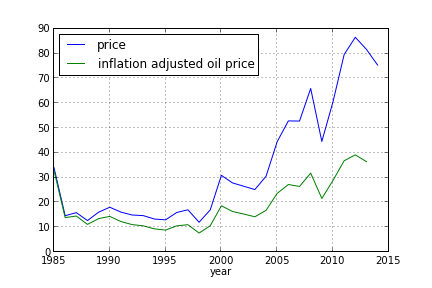
\includegraphics[height=6cm]{corr_05.png}

\begin{minted}[fontsize=\footnotesize]{python}
df['production'] = pd.read_csv('world.csv',index_col=0,sep=' ')
print df.production.corr(df['inflation adjusted oil price'])
print df[:10]
\end{minted}

\begin{verbatim}
0.644058365167
          price  inflation  inflation2  inflation adjusted oil price  \
year                                                                   
1985  33.998325        3.6    1.036000                     32.816916   
1986  14.634975        1.9    1.055684                     13.863026   
1987  15.872433        3.6    1.093689                     14.512753   
1988  12.671617        4.1    1.138530                     11.129806   
1989  16.059233        4.8    1.193179                     13.459195   
1990  18.053533        5.4    1.257611                     14.355420   
1991  16.085092        4.2    1.310431                     12.274661   
1992  14.916558        3.0    1.349744                     11.051402   
1993  14.665650        3.0    1.390236                     10.549037   
1994  13.295725        2.6    1.426382                      9.321293   

      production  
year              
1985       59.12  
1986       61.91  
1987       62.28  
1988       64.62  
1989       65.92  
1990       66.78  
1991       66.85  
1992       67.35  
1993       67.55  
1994       68.94  
\end{verbatim}























\end{document}
